\documentclass[conference]{IEEEtran}
\IEEEoverridecommandlockouts
% The preceding line is only needed to identify funding in the first footnote. If that is unneeded, please comment it out.
\usepackage{cite}
\usepackage{amsmath,amssymb,amsfonts}
\usepackage{algorithmic}
\usepackage{graphicx}
\usepackage{textcomp}
\usepackage{xcolor}
\usepackage{hyperref}
\def\BibTeX{{\rm B\kern-.05em{\sc i\kern-.025em b}\kern-.08em
    T\kern-.1667em\lower.7ex\hbox{E}\kern-.125emX}}
\begin{document}

\title{LEFIN-Filter\\
{\Large Line-rate Ethernet Frame Inline Network Filter}
}

\author{\IEEEauthorblockN{Luc Gaitskell}
    \IEEEauthorblockA{\textit{Electrical Engineering and Computer Science} \\
        \textit{Massachusetts Institute of Technology}\\
        Cambridge, MA, USA \\
        lucg@mit.edu}
    \and
    \IEEEauthorblockN{Noah Wiley}
    \IEEEauthorblockA{\textit{Electrical Engineering and Computer Science} \\
        \textit{Massachusetts Institute of Technology}\\
        Cambridge, MA, USA \\
        njwiley@mit.edu}
}

\maketitle

\begin{abstract}
    High speed Ethernet and encryption form the backbone of modern networks and data centers, routing and processing bigger data every day. It is vital to reject malicious attacks, but encryption aids in their disguise. Luckily, researchers have developed machine learning architectures capable of classifying encrypted packets from malicious programs with high accuracy. However, running these models on CPUs or GPUs on typical devices significantly bottleneck high speed 10G+ connections. We present a novel Line-rate Ethernet Frame Inline Network Filter (LEFIN-Filter) capable of performing classification and packet handling at line rate, introducing less than $1\mu S$ of latency with $99\%+$ accuracy on the USTC-TFC2016 dataset. We develop specially designed flexible hardware to implement effective models and tooling to train and test said models on an Ultrascale+ RFSoC ZU48DR platform.
\end{abstract}

\begin{IEEEkeywords}
    FPGA, Field Programmable Gate Artificial Intelligence (FPGAI), one-dimensional convolutional neural networks, encrypted traffic classification, network filter
\end{IEEEkeywords}

\section{Introduction}
Advances in data center technology and high speed Ethernet move and process extraordinary amounts of data per second while maintaining reliability and privacy. Hardware in routers and switches are highly optimized to route traffic as fast as possible. Encryption prevents eavesdroppers from stealing vital information. People and companies count on these features.

While most traffic is benign, system administrators must still monitor for malware to keep systems secure. Unfortunately, the very features that provide high speed and privacy make this more difficult for administrators. Encryption  aids bad actors in disguising the true content of their malicious data and packets. High speed routing leaves little time to perform complex inspections on packets.

Luckily, some, albeit nuanced, patterns exist in the encrypted data which can uniquely identify it with certain programs. Researchers, system administrators, and governments alike have turned to using machine learning models to aid in classification
\cite{paper-ensafi,paper-wang-conv1d}.
These models can achieve high accuracy, but their use for real-time filtering in high speed links is impractical, even with powerful servers, due to high overheads moving packets.
Moving the compute directly next to the
Ethernet Media Access Controller (MAC)
eliminates this limitation,
but is only possible in a custom hardware design.
This paper introduces such a hardware implementation,
which both classifies and handles packets at modern line rates.

\subsection{Classifying and Filtering Ethernet Frames}
The IEEE 802.3 standard defines Ethernet, a technology connecting devices everywhere today. Subsequent revisions and additional clauses have pushed bitrates higher and higher, with consumer devices now supporting bitrates up to 2.5 gigabits per second and modern data center links supporting speeds in excess of 10 Gbps per second per channel. At these speeds an average ethernet frame (791 Bytes) can be sent in 640 nanoseconds.

Ethernet operates on the 1st (Physical) and 2nd (Data) layer of the OSI model. For this project we focus on the second layer which Ethernet operates using frames as seen in Fig. \ref{fig:ether-frame}.

While the data payload field is often encrypted, encryption methods may be unique to certain programs (i.e. gmail, FaceTime, Cridex malware, Zeus malware). Therefore, accurate classification can be accomplished by individually inspecting entire frames with a convolutional neural network\cite{paper-wang-conv1d}. Finally, filtering can be accomplished by first classifying a frame as benign or malicious, then only propagating benign frames.
\begin{figure}
    \centering
    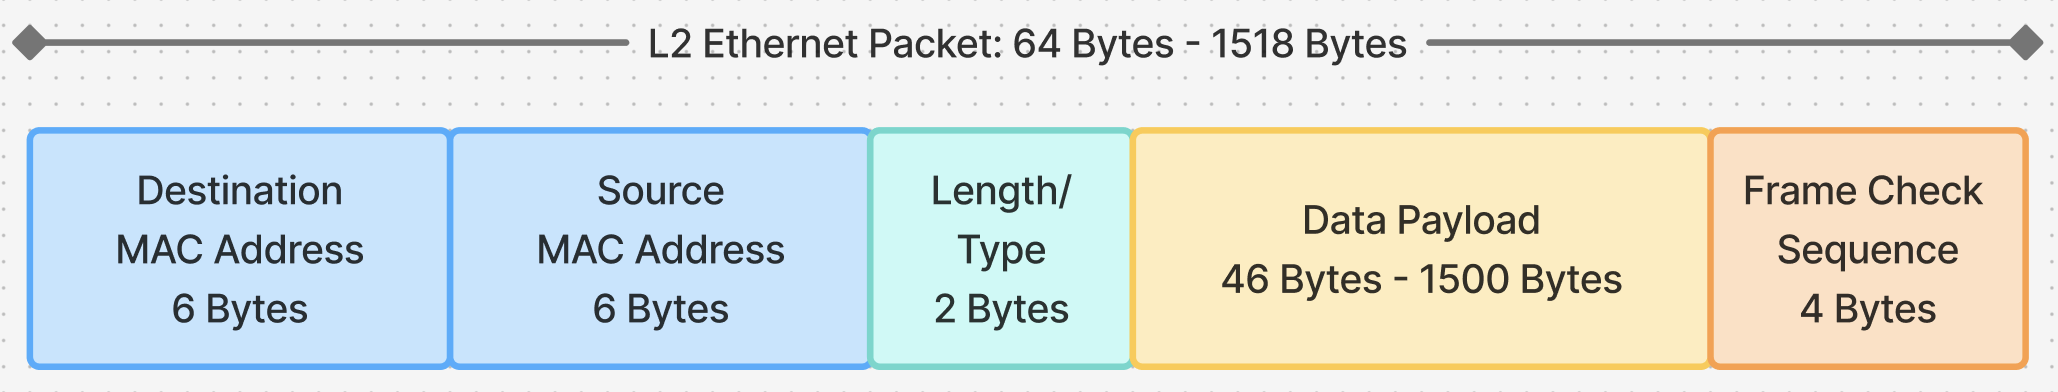
\includegraphics[width=1\linewidth]{images/ether_frame.png}
    \caption{Structure of an Ethernet Frame}
    \label{fig:ether-frame}
\end{figure}


\subsection{Challenges with a Server Implementation}
In a software packet filtering approach,
a server first needs to wait for the
Network Interface Card to copy the packet into
the system memory of the network filter server.
This requires the packet traversing the Network Interface Controller,
Peripheral Component Interconnect Express (PCIe)
interface, and finally being copied into system memory
before the CPU can begin executing the filter compute task.
Even in the most latency optimized configuration,
this still requires upwards of $3\mu$s before the
first byte can be processed \cite{paper-ix-os, paper-neugebauer}, with a similar latency on the outbound path. With some businesses measuring server latency in singular microseconds, the downsides outweigh the benefits of a system like this.

\subsection{Benefits of an FPGA}
Modern servers with software defined machine learning are flexible, but it comes at the cost of absolute speed. Baking logic into hardware allows routers and switches to achieve such high bitrates, but these devices become obsolete when a new standard is introduced. The task of network filtering demands the speed of hardware and the flexibility of software to effectively protect against evolving threats without imposing a bottleneck on critical links. Field Programmable Gate Arrays (FPGAs), oftentimes integrated on boards with ethernet and Quad Small Form-factor Pluggable (QSFP) ports, strike the perfect balance. FPGAs even allow for flexibility beyond model parameters (i.e. model architecture), also putting them a step ahead of ASICs. For this reason, LEFIN-Filter is implemented on an FPGA development board.

\subsection{Goals}
\begin{itemize}
    \item Classify and filter ethernet packets at 10 Gbps rate
    \item Provide deterministic predictable latency under $3\mu$s
    \item Achieve 95\% classification and filter accuracy
\end{itemize}

\subsection{Anticipated Challenges}
As with most machine learning models, demonstrated architectures, although small, rely on numerous floating point multiplies and accumulates (MACs). The model proposed by Wang et al.\cite{paper-wang-conv1d} would require an excess of 19 million of these operations which would still require a fully utilized advanced FPGA many cycles to perform. Additionally, ethernet is an intricate standard and imposes specific timing and ordering which our design must respect. Finally, the line rate of modern ethernet is extremely fast, and producing a system that can process every byte quickly and accurately will be difficult.

\subsection{Approach}
To accomplish our goals, we exploit a key feature of ethernet which acts as a speed bump to other systems, data transfer as a stream. While other systems have to wait many cycles for an entire frame to be transferred before processing, we aim to take advantage of these wasted to begin processing.

\section{Ethernet Frame Classification}

\subsection{Existing Research}
Existing research into network traffic classification
has yielded convolutional machine learning architectures
over the transmitted data.
Research into using these architectures has been used
for a wide range of traffic classification applications.
For example, classifying VPN and non-VPN traffic
of different application traffic flows \cite{paper-wang-conv1d}.
Although useful for analyzing general traffic usage on a network,
we chose instead to persue the other application:
classification of malicious and benign packets \cite{paper-wang-malware}.

Detecting malicious Ethernet frames at line rate would
allow a filter to immediately block such flows before they reach the user
or exit the networks.
For our filter, we chose the architecture of the
\textit{End-to-End encrypted traffic classification}
model \cite{paper-wang-conv1d},
with the data from the
\textit{Malware traffic classification} paper\cite{paper-wang-malware}.

\subsection{Data Processing}
The selected one-dimensional convolutional neural network (1D-CNN)
architecture \cite{paper-wang-conv1d},
was designed to convolve directly over the bytes of the network flow.
The existing research demonstrated evaluations at different selected
network levels, such as L7 or L3.

We elected to preprocess the packets as L2,
additionally separating each packet into distinct inputs
instead of combining them into flows.
This simulated the realistic use case of the network filter,
where multiple downstream devices would have separate
flows serially through this one device.

\subsection{Model Architecture}
Additionally, the existing research did not discuss modifications
to model architecture, and selected a standard model architecture:
% please insert something that looks okay here indicating:
% conv1d (1x25, stride=1, outchannels=32) -> maxpool (3, stride=3) -> relu -> conv1d (1x25, stride=1, outchannels=64) -> maxpool (3, stride=3) -> relu -> fully connected -> fully connected

% double check this:
As this model has $x$ trainable parameters,
it would have around $\sim40$Mb of weights, once int8 quantized.

This large size would be difficult for the synthesis and routing,
given the $38$Mb of BRAM and $22$Mb of UltraRAM,
and would give little headroom for other additions to the design.

The FPGA available for the project also has ample DDR4 available.
However, given a $1500$MB MTU of an Ethernet frame,
it would take around $1.2\mu$s to transmit through the wire at $10$G.
Given the RFSoC 4x2 DDR4 memory bandwidth of $19.2$GBps,
streaming the weights in would take over $250\mu$s,
which is far too slow for a line-rate design.

As a result, we focused on novel work to reduce and simplify the model
architecture, and settled on a significantly smaller design,
that still achieved near-perfect accuracy when trained and validated
on the malware dataset.
% conv1d (1x25, stride=1, outchannels=4) -> global max pool (4 channels) -> fully connected (4x2)

This shows that the dataset is highly separable,
and that a much less complex model is needed to classify the benign
and malicious packets of the dataset.

Similar to the original model architecture,
we chose to continue trimming or padding the packets
to be exactly $784$B of input.

\subsection{Quantization}
In order to encode the model weights into the FPGA,
we elected to use int8 weight quantization,
as it is a common choice for reducing unncessary
precision after training \cite{paper-int8}.

We utilize the widely used \texttt{torchao} library,
to quantize and export the weights to \texttt{int8}
\cite{paper-torchao}.
We built a script to export the weights from a quantized
checkpoint, generating a SystemVerilog header
with \texttt{localparam}s that specify the model parameters.

\subsection{Accuracy}
After training our new model architecture on the network
traffic dataset, we achieved a $99\%$ accuracy
on the de-duplicated validation set.
After int8 quantization, the accuracy maintained the same figure
within $0.1\%$.

\begin{figure}
    \centering
    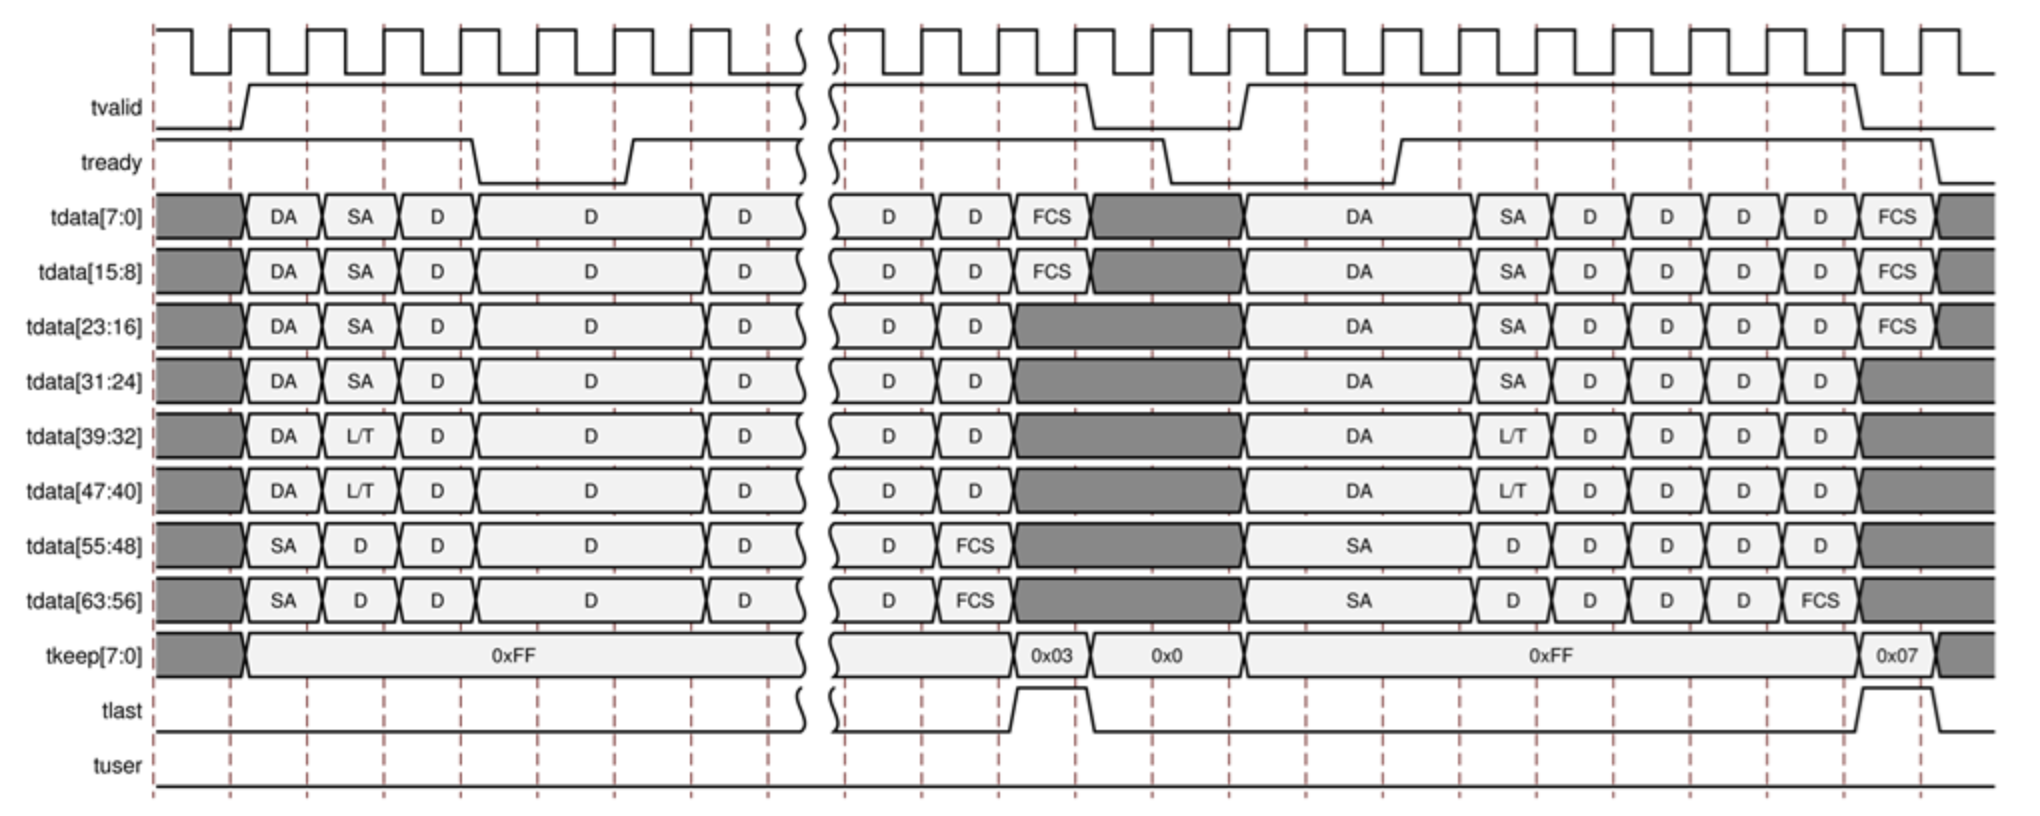
\includegraphics[width=1\linewidth]{images/ethernet_sub_tim.png}
    \caption{Example of Ethernet Subsystem AXI4-Stream}
    \label{fig:eth-sub-time}
\end{figure}
\subsection{RFSoC Capabilities and IP}\label{ref:sec-rfsoc-cap}
We implement our platform on the Real Digital RFSoC 4x2 development kit equipped with the UltraScale+ ZU48DR.
This FPGA platform is equipped with gigabit transceiver modules (GTY) built into the processing fabric.
With the addition of a QSFP port, this enables the use of the AMD 10G/25G High Speed Ethernet Subsystem IP providing an intuitive way to connect our filter
inline to the stream of Ethernet frames.
This IP core handles the MAC and Physical Coding Sublayer (PCS),
and provides a AXI4-Stream interface for both the TX and RX datapaths.

The module interfaces are clocked at the GT reference clock of $156.25$MHz.
The AXI4-Streams are provided as a 64b bus, transferring $8$ new bytes
of the Ethernet frame each cycle, as seen in Fig. \ref{fig:eth-sub-time}.

\section{LEFIN-Filter Logical Design}
\begin{figure}
    \centering
    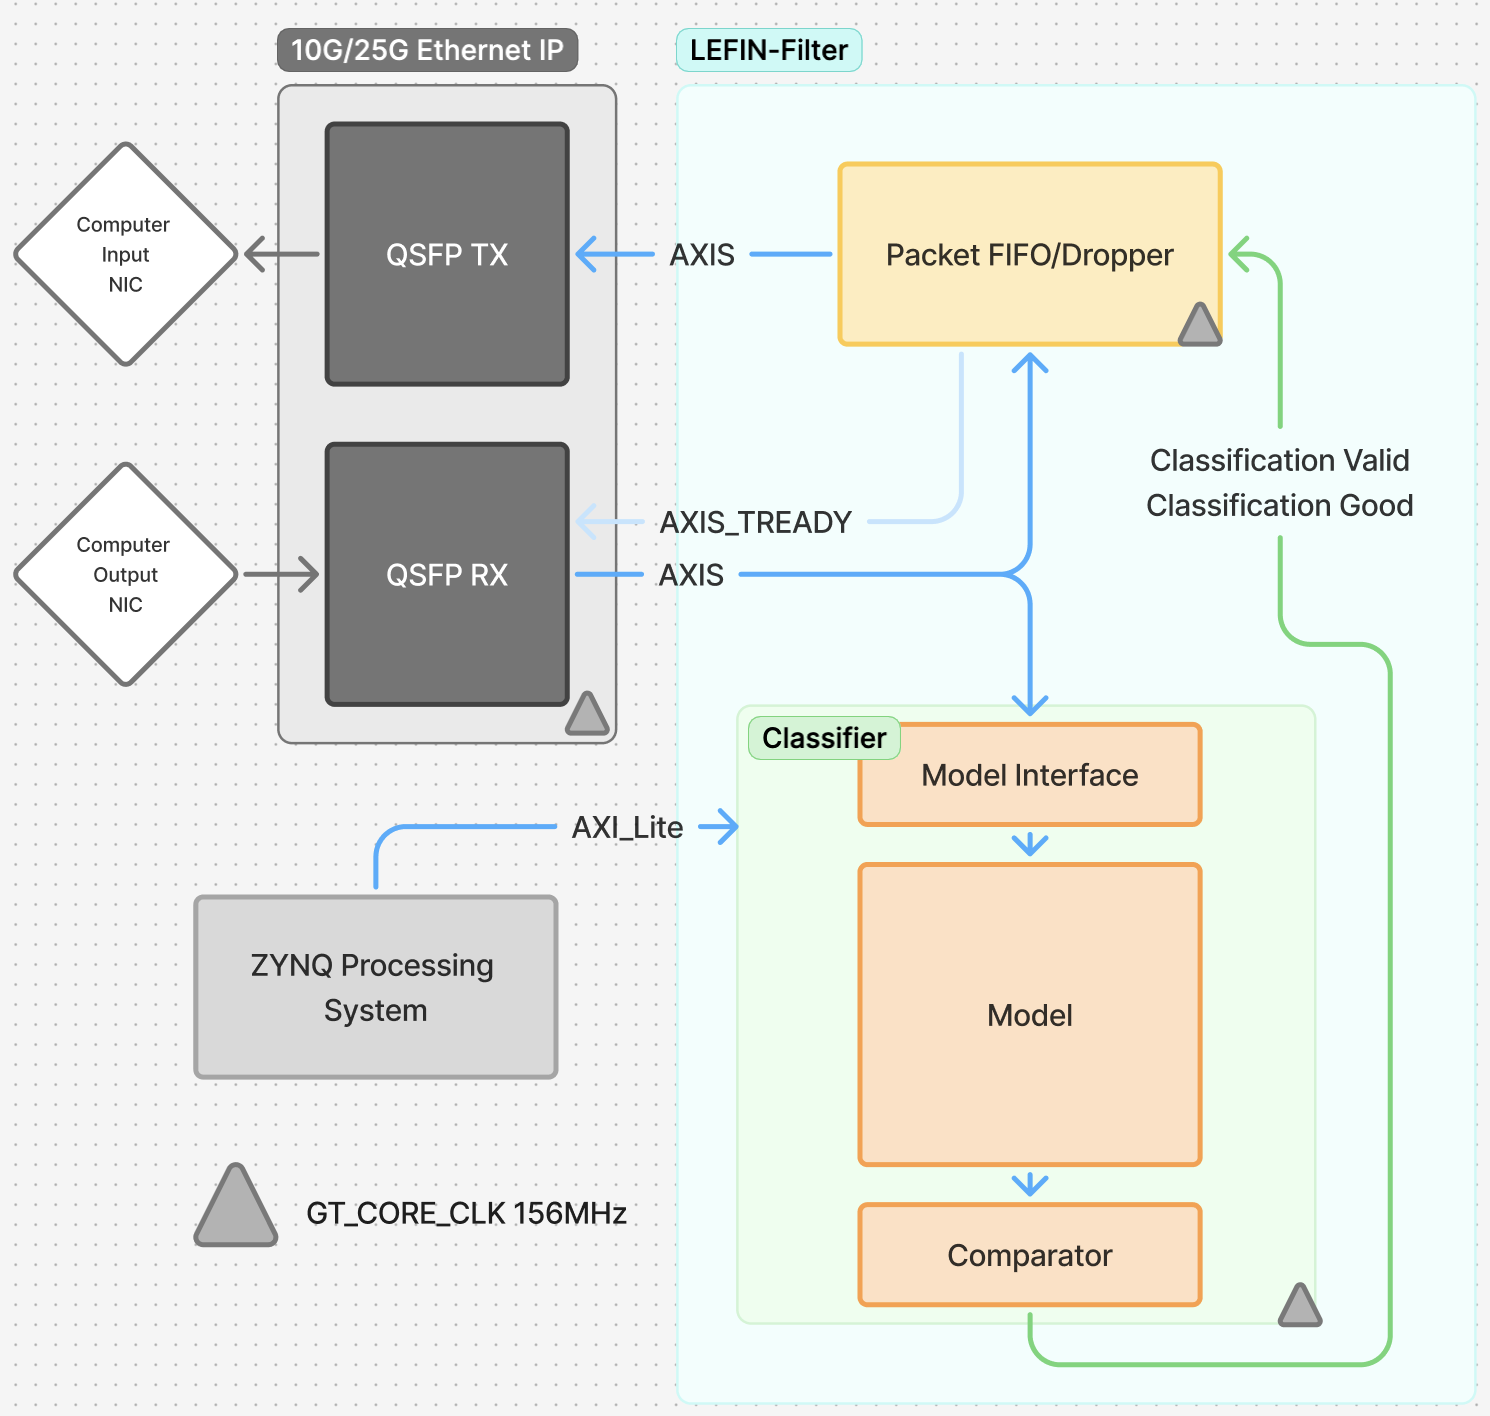
\includegraphics[width=1\linewidth]{images/general_bd.png}
    \caption{General Block Diagram of Filter}
    \label{fig:gen_bd}
\end{figure}

The LEFIN-Filter implementation is packaged as an individual IP,
designed to be directly connected to the TX and RX interfaces on
the Ethernet Subsystem IP core.
For future flexibility, a AXI4-Lite interface is also included
to allow future external configuration or access to internal state.

Our filter operates as follows:
\begin{enumerate}
    \item The Ethernet IP begins to stream a new packet to the
          FIFO and the classifier simultaneously.
    \item The FIFO continuously accumulates the packet bytes
    \item The FIFO computes the layer activations continuously on the stream.
    \item Once the classifier outputs a single-cyle classification signal,
          the FIFO acts accordingly to begin emptying to the Ethernet TX
          or drops the packet entirely.
\end{enumerate}
A high level diagram is included in Fig. \ref{fig:gen_bd}.

\subsection{Module Interconnects and Clock}

To maintain modularity and portability,
we designed our modules to use AXI4-Stream interfaces.
This unifies the test bench designs,
and makes it possible and simple to connect any layer to another.

Additionally, all modules run on the GT core clock,
as the Ethernet IP RX and TX interfaces are on the same clock domain.

\subsection{Classifier}
\begin{figure}
    \centering
    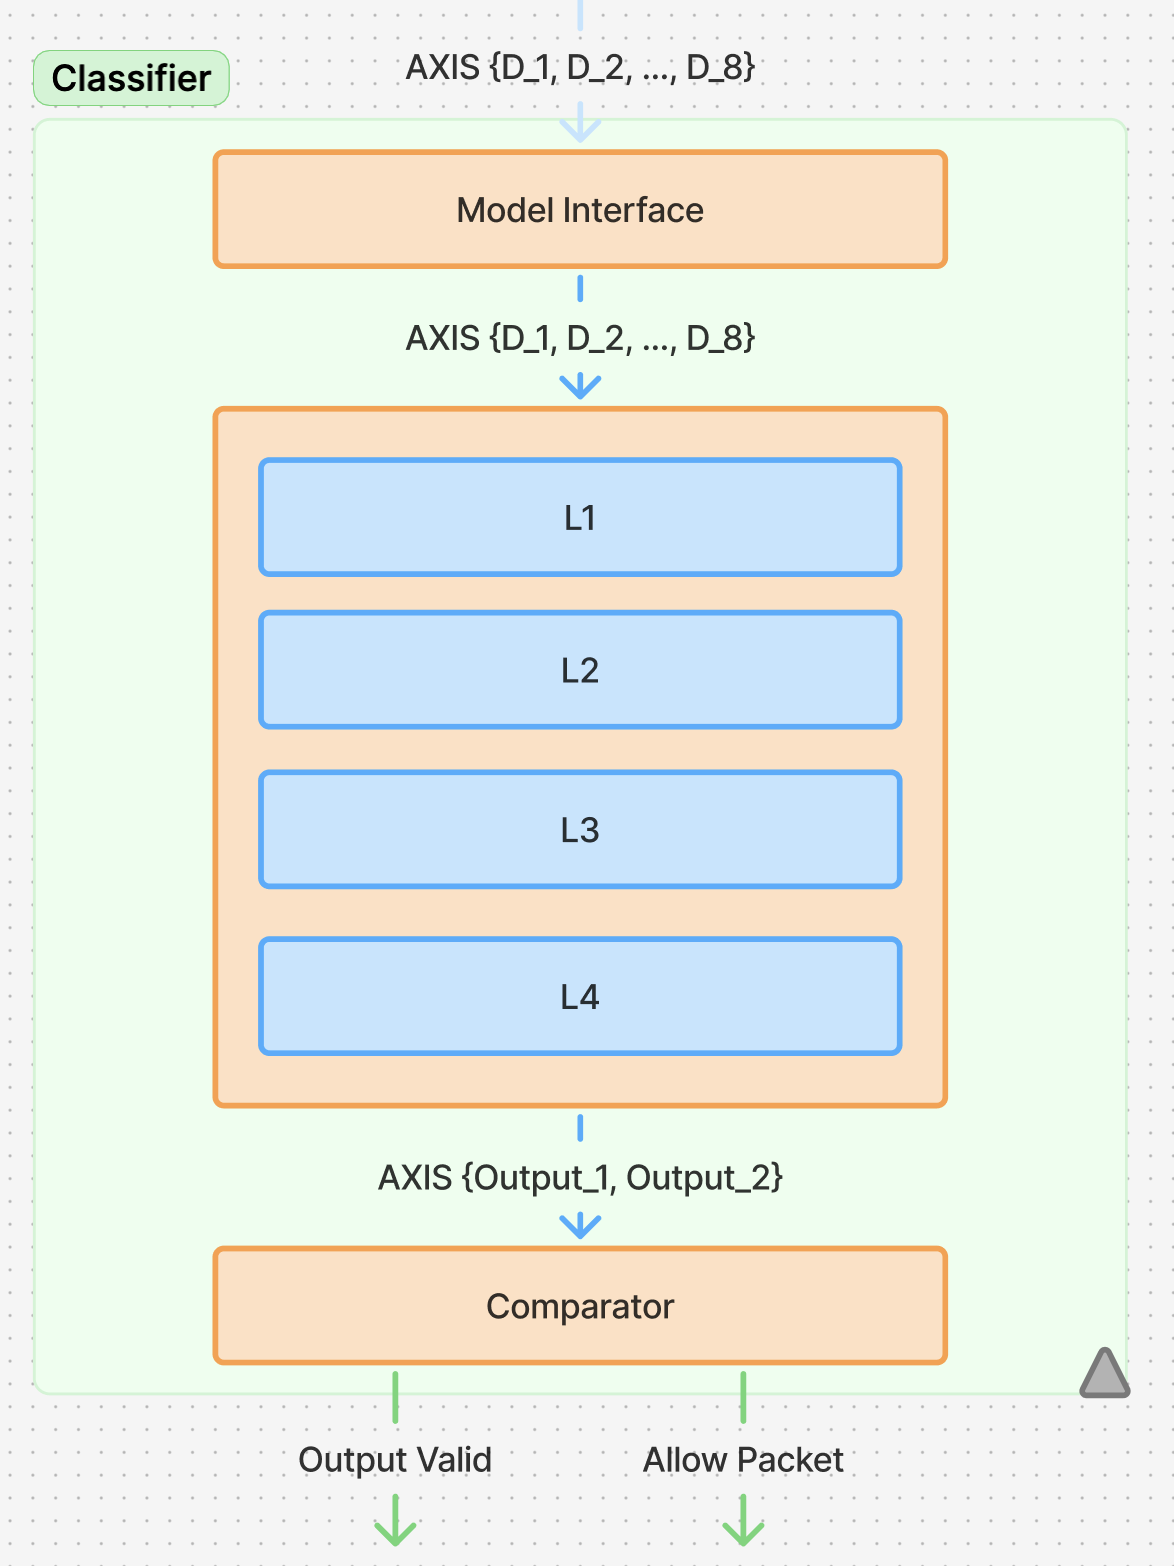
\includegraphics[width=0.7\linewidth]{images/classifier.png}
    \caption{Classifier Structure}
    \label{fig:classifier}
\end{figure}
\begin{figure}
    \centering
    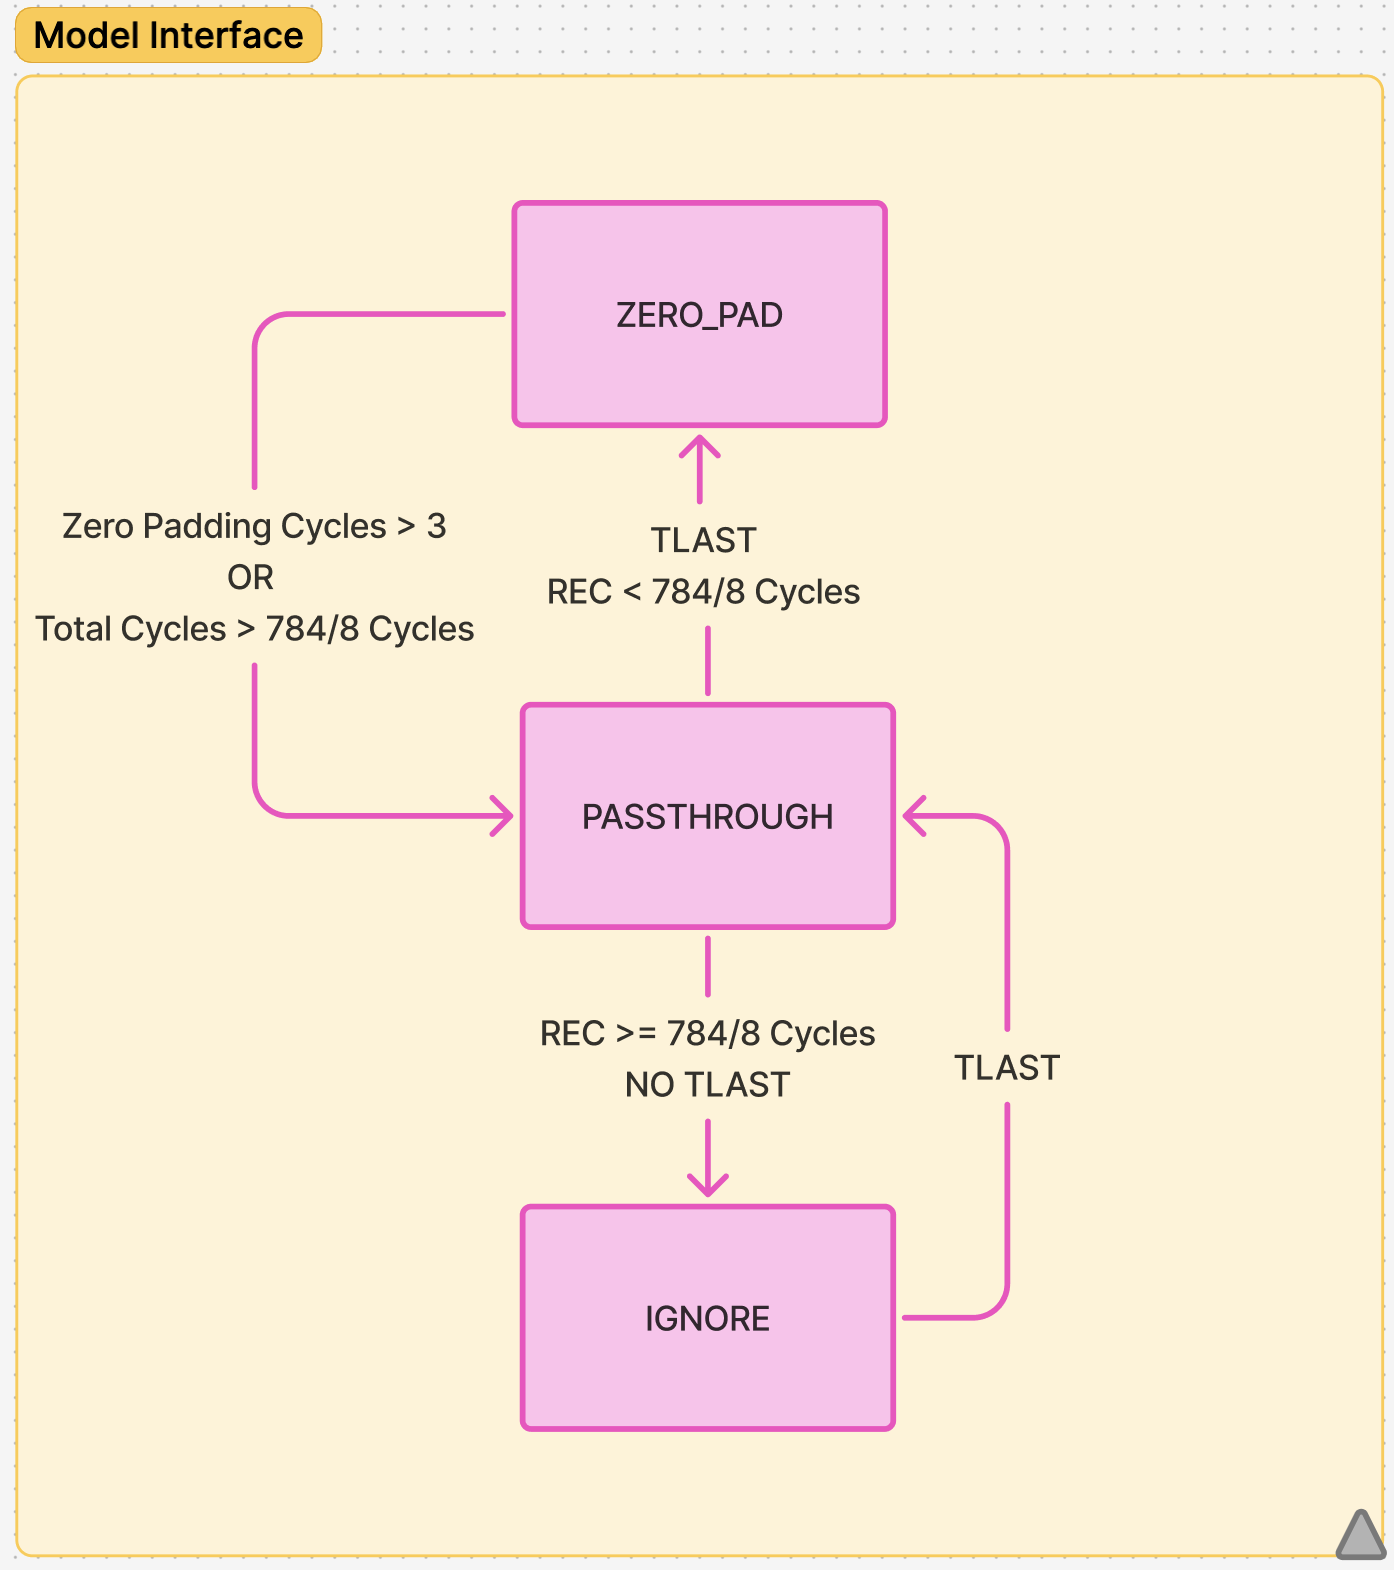
\includegraphics[width=0.7\linewidth]{images/model_inter_fsm.png}
    \caption{Model Interface FSM}
    \label{fig:mod-inter-fsm}
\end{figure}
The classifier directly interfaces with the AXI4-Stream,
interface of the Ethernet Subsystem IP.
The structure of the classifier is shown in Figure \ref{fig:classifier}.

\subsubsection{Model Interface}
The model interface prepares the Ethernet frame stream for the model.
In order to strictly match the logical behavior of the
model as it was trained and validated in software,
we only pass a maximum of $784$B from the frame
to the model.
After this threshold is reached,
we continue to exhaust and ignore the upstream bytes
from the Ethernet Subsystem to clear the AXI4-Stream.
Additionally, for packets shorter than this requirement,
we pad the outputs to match the padding in software.
To avoid an unnecessary number of zero padded cycles,
we limit this purging to 3 cycles,
which adds at least 24 padded inputs to complete the
convolution of the 25 wide convolution kernel.
The end of the packet is delineated by a \texttt{tlast} signal from
the Ethernet Subsystem,
and the clipped or padded packet end
is also propagated to the model as a \texttt{tlast}.
This process is described in Figure \ref{fig:mod-inter-fsm}.

\subsubsection{Model}
The model is a pure wrapper around a collection of model layers,
described below in section \ref{ref:model-layers}.

\subsubsection{Comparator}
The final classification layer in the model outputs the activations,
in a single cycle, over the model AXI4-Stream output.
The larger output value indicates the more probable class for the
classification.
This comparison is indicated as simple valid signal
with a classification value bit.

\subsection{Model Layers}\label{ref:model-layers}
The inputs and outputs are packed AXI4-Stream buses,
in the standardized pattern set out in pytorch's \texttt{tensor.flatten()}.
% Format this as something nice in the middle (I don't want it wrapped)
% \texttt{[OUT CHANNEL][IN CHANNEL][INPUT WIDTH]}

This allows interfacing between different types of layers,
such as ReLU, which is shape agnostic.
Additionally, using a packed structure follows the standard
AXI spec and makes it easier to interface with other IP if necessary.

All models are parameterized with the input bit widths,
along with the shape of the input if relevant.

\subsubsection{1D Convolution}
As the Ethernet Subsystem data stream delivers 8 inputs per cycle,
we are able to evaluate 8 simultaneous convolutions.
Given the kernel width of 25, we retain the 24 previous inputs,
continually updating it as we receive new inputs over the bus.
As a result, the first 3 cycles (of 8 inputs) do not produce activations,
and just fill the input buffer.
Each convolution has a single activation,
yielding an output bus with the same number of values,
although with an increased bit width to match the result
of the multiply accumulates.

Given the timing constraints on the RFSoC board,
we made the convolution a 2 cycle pipelined design:
\begin{enumerate}
    \item Multiply kernel with inputs
    \item Half-reduce the outputs to two sums
    \item Add the final two sums combinationally
\end{enumerate}

The convolutions support just a single channel as input,
but support a fully customizable number of output channels.

\subsubsection{ReLU}
This layer is a combinational $\text{min}(0, x)$ on the inputs.

\subsubsection{Global Maximum Pool}
The global maximum pooling (GMP) layer evaluates the maximum value
in a channel.
The maximum value is computed and retained each cycle,
as new inputs are provided.
The resulting maximum values, for each channel,
are only propagated to the following layer once a \texttt{tlast}
is received on the input.

\subsubsection{Fully Connected}
The full connected layer can be summarized as a single matrix multiply followed by an add with a bias term. Our implementation receives inputs through an AXI4-Stream bus and a weights and biases input channel. We use the same packing standard for weights, biases, and inputs as our Conv1D Layer.
Given the relatively small output size of the global max pool layer, this layer is implemented entierely combinationally, reducing the latency of our system. It first splits the inputs, multiplies them by their weights, and adds the results with their respective biases. It outputs the results as a packed array on an AXI4-Stream Bus.
\subsection{Drop Buffer FIFO}
The drop buffer FIFO is responsible for either propagating or dropping packets as well as providing back pressure to the ethernet subsystem. It takes in an AXI4-Stream from the receive side of the ethernet subsystem and outputs an AXI4-Stream bus to the transmit side of the ethernet sub system. Additionally, it receives two control signals $valid$ and $good$ which in combination with the $tlast$ signal from the AXI4-Stream S port, implements the FSM seen in Fig. \ref{fig:fifo_fsm}. If a frame is dropped the pipeline can begin processing the next frame immediately. If the frame is propagated, the filter can begin processing the next frame when the FIFO is empty.
\begin{figure}
    \centering
    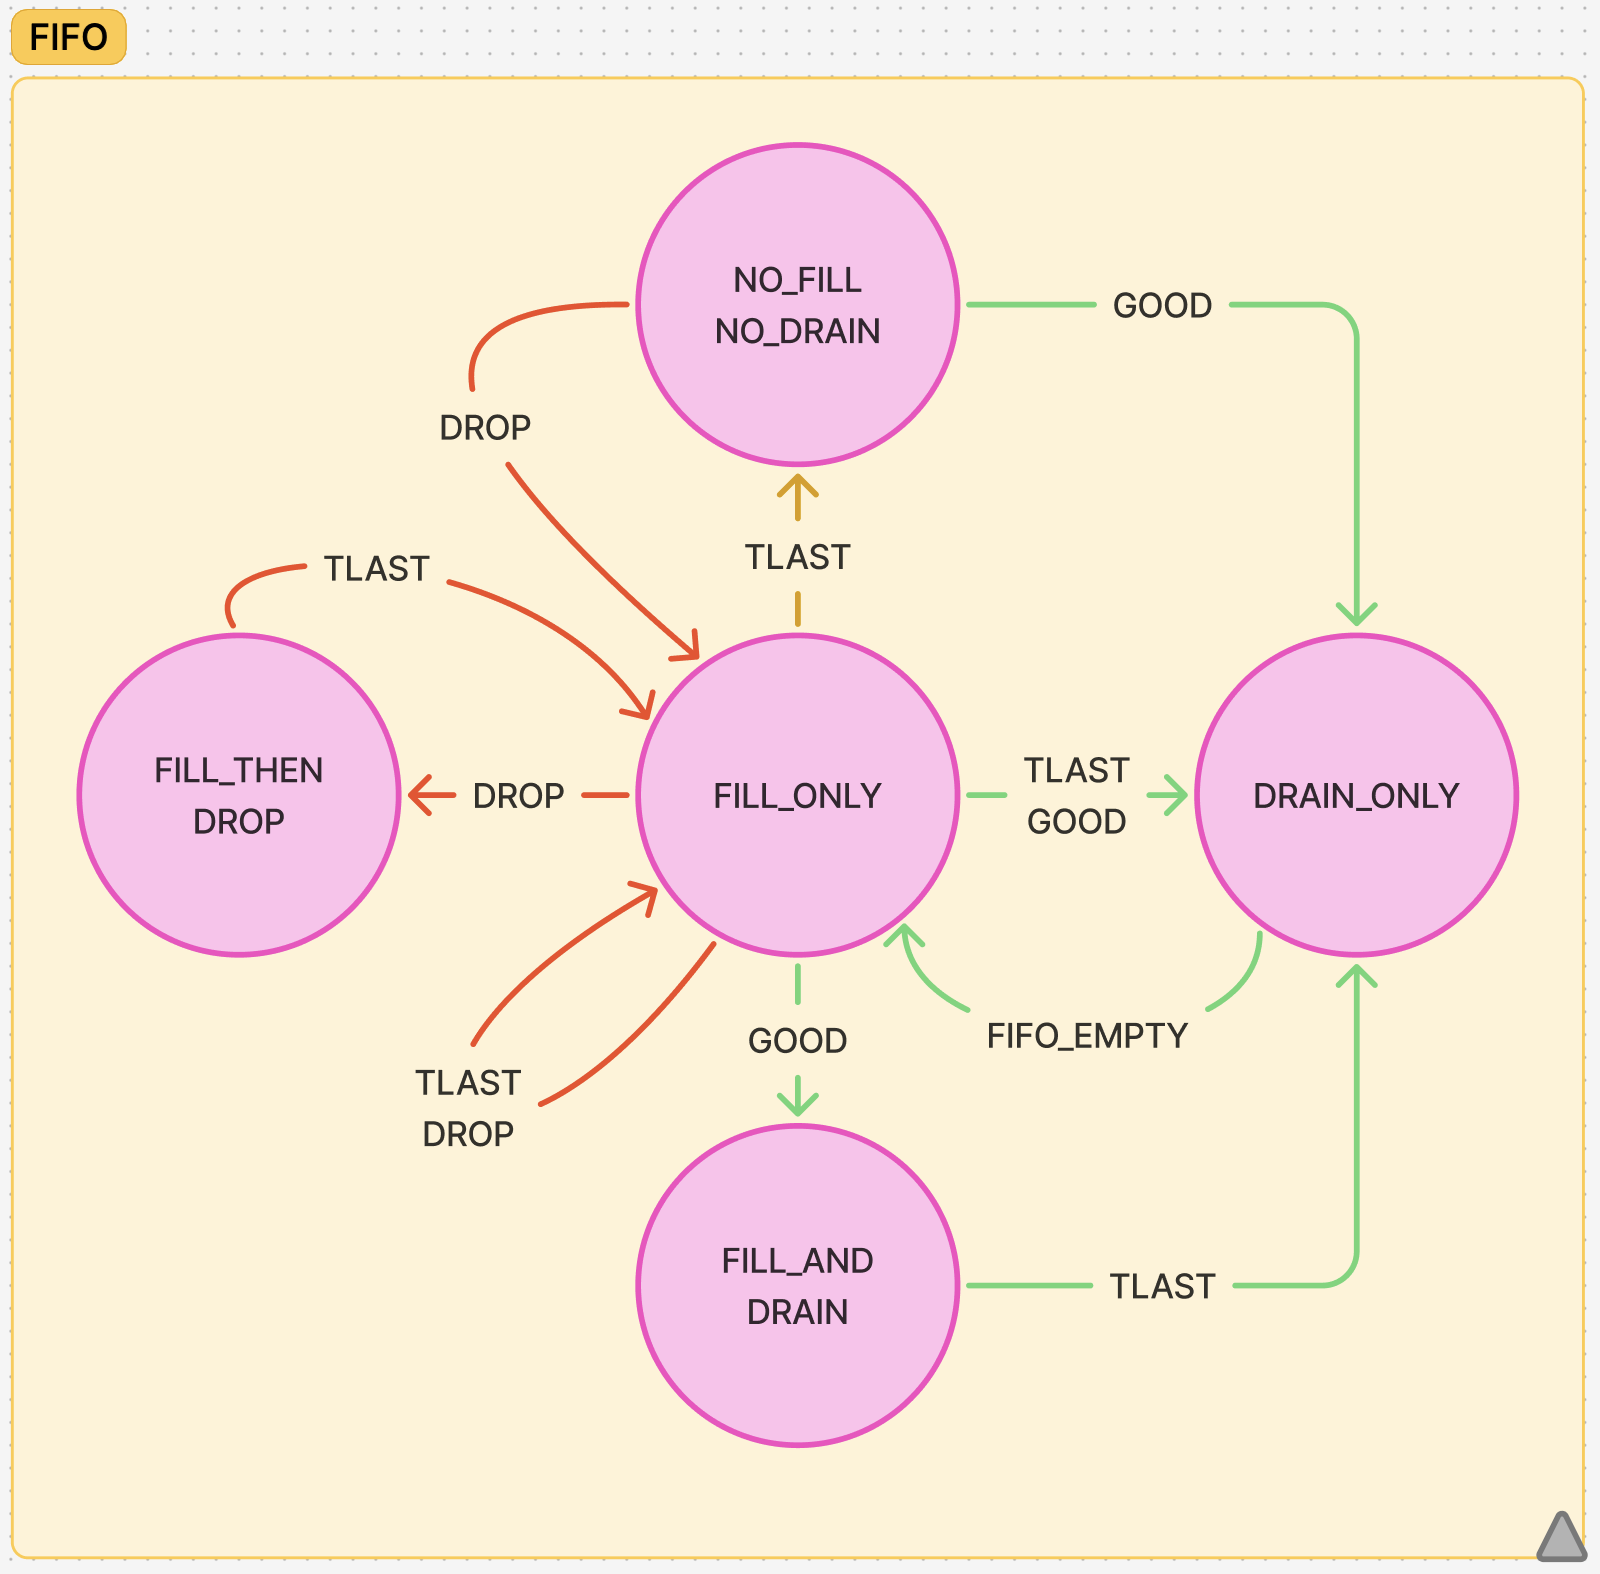
\includegraphics[width=0.7\linewidth]{images/fifo_fsm.png}
    \caption{Drop Buffer FIFO FSM}
    \label{fig:fifo_fsm}
\end{figure}


\section{Simulation}

\subsection{Testbenching: Model Layers}
To validate the model layer designs,
they are all individually tested against the PyTorch implementations,
on randomized inputs.
As all layers implement a AXI4-Stream interfaces both for inputs
and outputs, the testbench harnesses have been generalized and shared.

\subsection{Testbenching: Full Model}\label{ref:tb-full-model}
After the model has been trained, the model parameters are quantized
and assigned in the model hdl.
The full model testbench allows verification of the
integration of these layers.
Although PyTorch does not support evaluation with
integer inputs and activations,
the integer weights yield activations that can be compared
directly with the output of the hardware design, with tolerance.

\subsection{Testbenching: Classifier}\label{ref:tb-classifier}
To test the classifier, the testbench is similar to
that in Section \ref{ref:tb-full-model},
but uses specific packet inputs from the test dataset.
This provides a higher level integration test,
and also is a sanity check for model classification behavior
compared to the software model.

\subsection{Testbenching: Full Integration}
The entire LEFIN-Filter IP additionally has a testbench,
similar to Section \ref{ref:tb-classifier},
which uses data from the test dataset.
This verifies that the correct packets,
as classified by the software model,
are rejected or passed through.

\section{Evaluation}
\begin{figure}
    \centering
    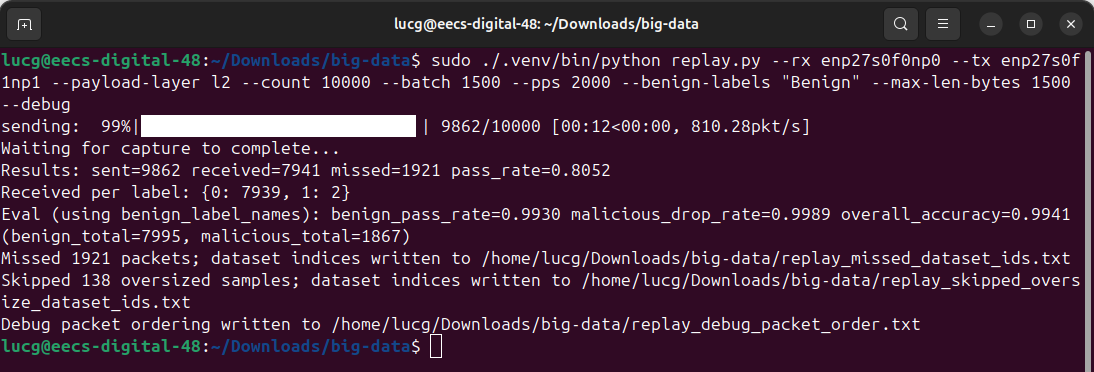
\includegraphics[width=1\linewidth]{images/accuracy_test.png}
    \caption{Classification accuracy test at our NIC's maximum rate}
    \label{fig:accuracy-run}
\end{figure}
We set up a simulated environment to test our design on the RFSoC 4x2.

\subsection{Demonstration Platform}
To evaluate the performance and accuracy of LEFIN-Filter,
we used a MIT EECS Lab Computer, with a
Mellanox ConnectX-4 Lx EN (MCX4121A-ACAT) NIC.
We used a standard Direct Attach Copper (DAC)
QSFP28 to 4xSFP28 cable, connecting one channel
to each interface on the NIC.

When configuring the Ethernet Subsystem IP,
described in Section \ref{ref:sec-rfsoc-cap},
we configured and connected the core
recieve and transmit on the same core,
which uses a single interface.
This is due to the QSFP wiring on the RFSoC 4x2
board, as the TX and RX channels are paired in reverse,
per-GT:
\begin{itemize}
    \item TX1 is with RX4
    \item TX2 is with RX3
    \item TX3 is with RX2
    \item TX4 is with RX1
\end{itemize}
Unfortunately, this makes it impossible to use the
Ethernet Subsystem IP with just a single channel.
However, for our testing we enabled GT 1 and 4
in the IP to enable SFP
channel 1 and 4 at the same time.

\subsection{Dataset}
We run our real world demonstration and evaluation using the
\href{https://github.com/davidyslu/USTC-TFC2016}{USTC-TFC2016}
dataset which consists of a collection of pcap files of captured raw network packets from various programs seen in Table \ref{tab:dataset}. At the beginning of the project we generate a training and validation split of 9:1 which we kept constant throughout training and testing.

\begin{figure}
    \centering
    \begin{tabular}{cccc}
        \textbf{Benign} & \textbf{Malware} & \textbf{Benign} & \textbf{Malware} \\
        BitTorrent      & Cridex           & Outlook         & Nsis             \\
        Facetime        & Geodo            & Skype           & Shifu            \\
        FTP             & Htbot            & SMB             & Tinba            \\
        Gmail           & Miuref           & Weibo           & Virut            \\
        MySQL           & Neris            & Warcraft        & Zeus             \\
        \\
    \end{tabular}
    \caption{USTC-TFC2016 Dataset}
    \label{tab:dataset}
\end{figure}

\subsection{Results}
\subsubsection{Accuracy}
To evaluate accuracy, we send Ethernet frames from the
validation split of the dataset from one network interface
and record the packets recieved on the other interface.
This allows the evaluation script to determine the accuracy,
in terms of dropped malicious frames and benign packets
that are successfully passed through.
The test script was limited at sending at most $\sim800$ packets
per second, likely due to a limitation between
\texttt{scapy}, Python, the operating system, or the NIC drivers.

\begin{figure}
    \centering
    \begin{tabular}{cccc}
                              & \textbf{Benign} & \textbf{Malware} \\
        \textbf{Received}     & 23683           & 6                \\
        \textbf{Total}        & 23860           & 3439             \\
        \textbf{Receive rate} & 99.26\%         &                  \\
        \textbf{Drop rate}    &                 & 99.83\%
    \end{tabular}
    \caption{Hardware evaluation run with $\sim30$k test frames}
    \label{tab:results-accuracy}
\end{figure}

As demonstrated in the software \texttt{pytorch} model,
we achieved over a $99\%$ accuracy.
An example classification test is shown in Figure \ref{fig:accuracy-run}.
Additionally, a larger test using $\sim30$k of the $\sim98$k test frames
demonstrated the high accuracy with results in table \ref{tab:results-accuracy}.

\subsubsection{Latency}
To evaluate latency, we hoped to build a script to use
hardware timestamping on the NIC to track the packet TX
and RX times with sufficient precision and accuracy.
In order to avoid the filter from tampering with the results,
we re-synthesized with the classification output wired to zero (benign).
However, this is still a fair evaluation of our demonstration,
as the FIFO still has to wait to forward the packet until the valid
signal from the model is high for one cycle.
This allows each test packet to always be forwarded,
but still had the added latency of waiting for the classifier output.
We compared latency to a reference design,
which matches the integration block diagram
in Figure \ref{fig:integration-block-diagram},
with the LEFIN-Filter module replaced with a Xilinx FIFO IP.

\begin{figure}
    \centering
    \begin{tabular}{cccc}
                         & \textbf{Reference Design} & \textbf{LEFIN-Filter} \\
        \textbf{Minimum} & $10.27\mu$s               & $10.25\mu$s           \\
        \textbf{Maximum} & $10.31\mu$s               & $10.31\mu$s           \\
        \textbf{Average} & $10.29\mu$s               & $10.28\mu$s
    \end{tabular}
    \caption{Recorded latency timing between Ethernet Subsystem passthrough reference design vs LEFIN-Filter}
    \label{tab:results-latency}
\end{figure}

However, we were unable to successfully run a script
that monitored the two interfaces while also supporting
hardware timestamping.
We were able to use the \href{tools/testing/selftests/net/timestamping.c}
{\texttt{timestamping.c} selftest from the linux kernel}
to send packets and manually collect TX timestamps,
at a 5s interval.
We then ran \texttt{tcpdump} with the flags
\texttt{--time-stamp-precision=nano} and
\texttt{-j adapter\_unsynced}
on the other interface to attempt to collect hw timestamps.
We compared the timing of our full LEFIN-Filter implementation,
shown in Figure ,
against a passthrough reference design, shown in Figure .

The results shown in table \ref{tab:results-latency} show
that we are unable to measure the latency with our current setup.
Additionally, it indicates that the timestamping script and/or
\texttt{tcpdump} is likely not using HW timestamps.

\section{Discussion}
\subsection{Implementation report}
\begin{figure}
    \centering
    \begin{tabular}{cccc}
        \textbf{Resource} & \textbf{Utilization} & \textbf{Available} & \textbf{Utilization \%} \\
        LUT               & 42626                & 425280             & 10.0                    \\
        LUTRAM            & 2822                 & 213600             & 1.3                     \\
        FF                & 29746                & 850560             & 3.5                     \\
        BRAM              & 8                    & 1080               & 0.74                    \\
        DSP               & 7                    & 4272               & 0.16                    \\
        GT                & 2                    & 16                 & 12.5
    \end{tabular}
    \caption{Vivado Implementation Report}
    \label{tab:imp_rep}
\end{figure}

The FPGA resource utilization, shown in Figure \ref{tab:imp_rep}
is relatively low for multiple reasons:
\begin{itemize}
    \item The model is small
    \item The model parallelism is limited by the
          AXI4-Stream width from the Ethernet Subsystem IP
    \item The weights are defined at synthesis time
\end{itemize}

\section{Future Work}
\subsection{Non-Blocking FIFO or FCS Corruption}
In scenarios with back to back frame transfers from the ethernet subsystem, our Drop Buffer FIFO may cause a back log if it needs to finish propagating a large packet. Although, we were far from reaching this limit and unable to observe this with our demonstration platform, we believe it could be beneficial to proactively address this. To minimize the chances of this backlog, we can implement a variety of solutions ranging from duplicating the FIFO and adding an arbiter for the active FIFO, creating a FIFO which holds and marks more frames, or by adding FCS corruption to minimize delay.

\subsection{More Types of Classifications}
Malware is ever evolving. While the current model architecture is sufficient for identifying the malware vs benign frames, expanding our layers and adding softmax may allow us to classify certain types of malware or types of benign frames.

\subsection{Live Weight Updates and Multi-Model Selection}
While our model layers take in variable weights, they are currently set at synthesis time. Additionally, with the low utilization of a single model, we could easily fit different models on the FPGA. The filter's AXI4-Lite port could be used to modify weights and select parameters from the processing system layer, removing the need to reflash the FPGA to modify the model.

\subsection{Diagnostics}
Currently there is no diagnostic or performance data collected
on device. Such performance counters could allow the model,
or multiple models, to be evaluated for their accuracy.
Additionally a sub-sample of rejected or allowed packets
could be redirected to the host memory through DMA for later review.

\section{Acknowledgments}
We would like to thank Joe Steinmeyer and Oliver Trevor for their assistance, support, and for making 6.S965 a very interesting and enjoyable class!


\begin{thebibliography}{00}
    \bibitem{paper-ensafi} Ensafi, Roya, et al. "Examining how the Great Firewall discovers hidden circumvention servers." Proceedings of the 2015 Internet Measurement Conference. 2015.
    \bibitem{paper-wang-conv1d} {W. Wang, M. Zhu, J. Wang, X. Zeng and Z. Yang, "End-to-end encrypted traffic classification with one-dimensional convolution neural networks," 2017 IEEE International Conference on Intelligence and Security Informatics (ISI), Beijing, China, 2017, pp. 43-48, doi: 10.1109/ISI.2017.8004872.}
    \bibitem{paper-neugebauer}Neugebauer, Rolf, et al. "Understanding PCIe performance for end host networking." Proceedings of the 2018 Conference of the ACM Special Interest Group on Data Communication. 2018.
    \bibitem{paper-ix-os} {Adam Belay, George Prekas, Mia Primorac, Ana Klimovic, Samuel Grossman, Christos Kozyrakis, and Edouard Bugnion. 2016. The IX Operating System: Combining Low Latency, High Throughput, and Efficiency in a Protected Dataplane. ACM Trans. Comput. Syst. 34, 4, Article 11 (January 2017), 39 pages. https://doi.org/10.1145/2997641}
    \bibitem{paper-wang-malware}{Wei Wang, Ming Zhu, Xuewen Zeng, Xiaozhou Ye and Yiqiang Sheng, "Malware traffic classification using convolutional neural network for representation learning," 2017 International Conference on Information Networking (ICOIN), Da Nang, Vietnam, 2017, pp. 712-717, doi: 10.1109/ICOIN.2017.7899588.}
    \bibitem{ref-eth-sub}AMD 10G/25G High Speed Ethernet Subsystem https://docs.amd.com/r/en-US/pg210-25g-ethernet/Introduction?tocId=reO6WKaRxFuxiCk6fDpLBQ
    \bibitem{paper-torchao}{Or, Andrew, Apurva Jain, Daniel Vega-Myhre, Jesse Cai, Charles David Hernandez, Zhenrui Zheng, Driss Guessous, Vasiliy V. Kuznetsov, Christian Puhrsch, Mark-Albert Saroufim, Supriya Rao, Thien Tran and Aleksandar Samardzic. “TorchAO: PyTorch-Native Training-to-Serving Model Optimization.” ArXiv abs/2507.16099 (2025).}
    \bibitem{paper-int8}{Wu, Hao, Patrick Judd, Xiaojie Zhang, Mikhail Isaev and Paulius Micikevicius. “Integer Quantization for Deep Learning Inference: Principles and Empirical Evaluation.” ArXiv abs/2004.09602 (2020).}
\end{thebibliography}


\appendix
\subsection{Source Code}
We have made the project artifact available on Github:
\href{https://github.com/luciengaitskell/lefin-filter}{https://github.com/luciengaitskell/lefin-filter}
\subsection{Vivado Block Diagram}
A toplevel Vivado block diagram of our system with the 10G/25G Ethernet Subsystem is included in Figure \ref{fig:integration-block-diagram}

\begin{figure*}[htbp]
    \centering
    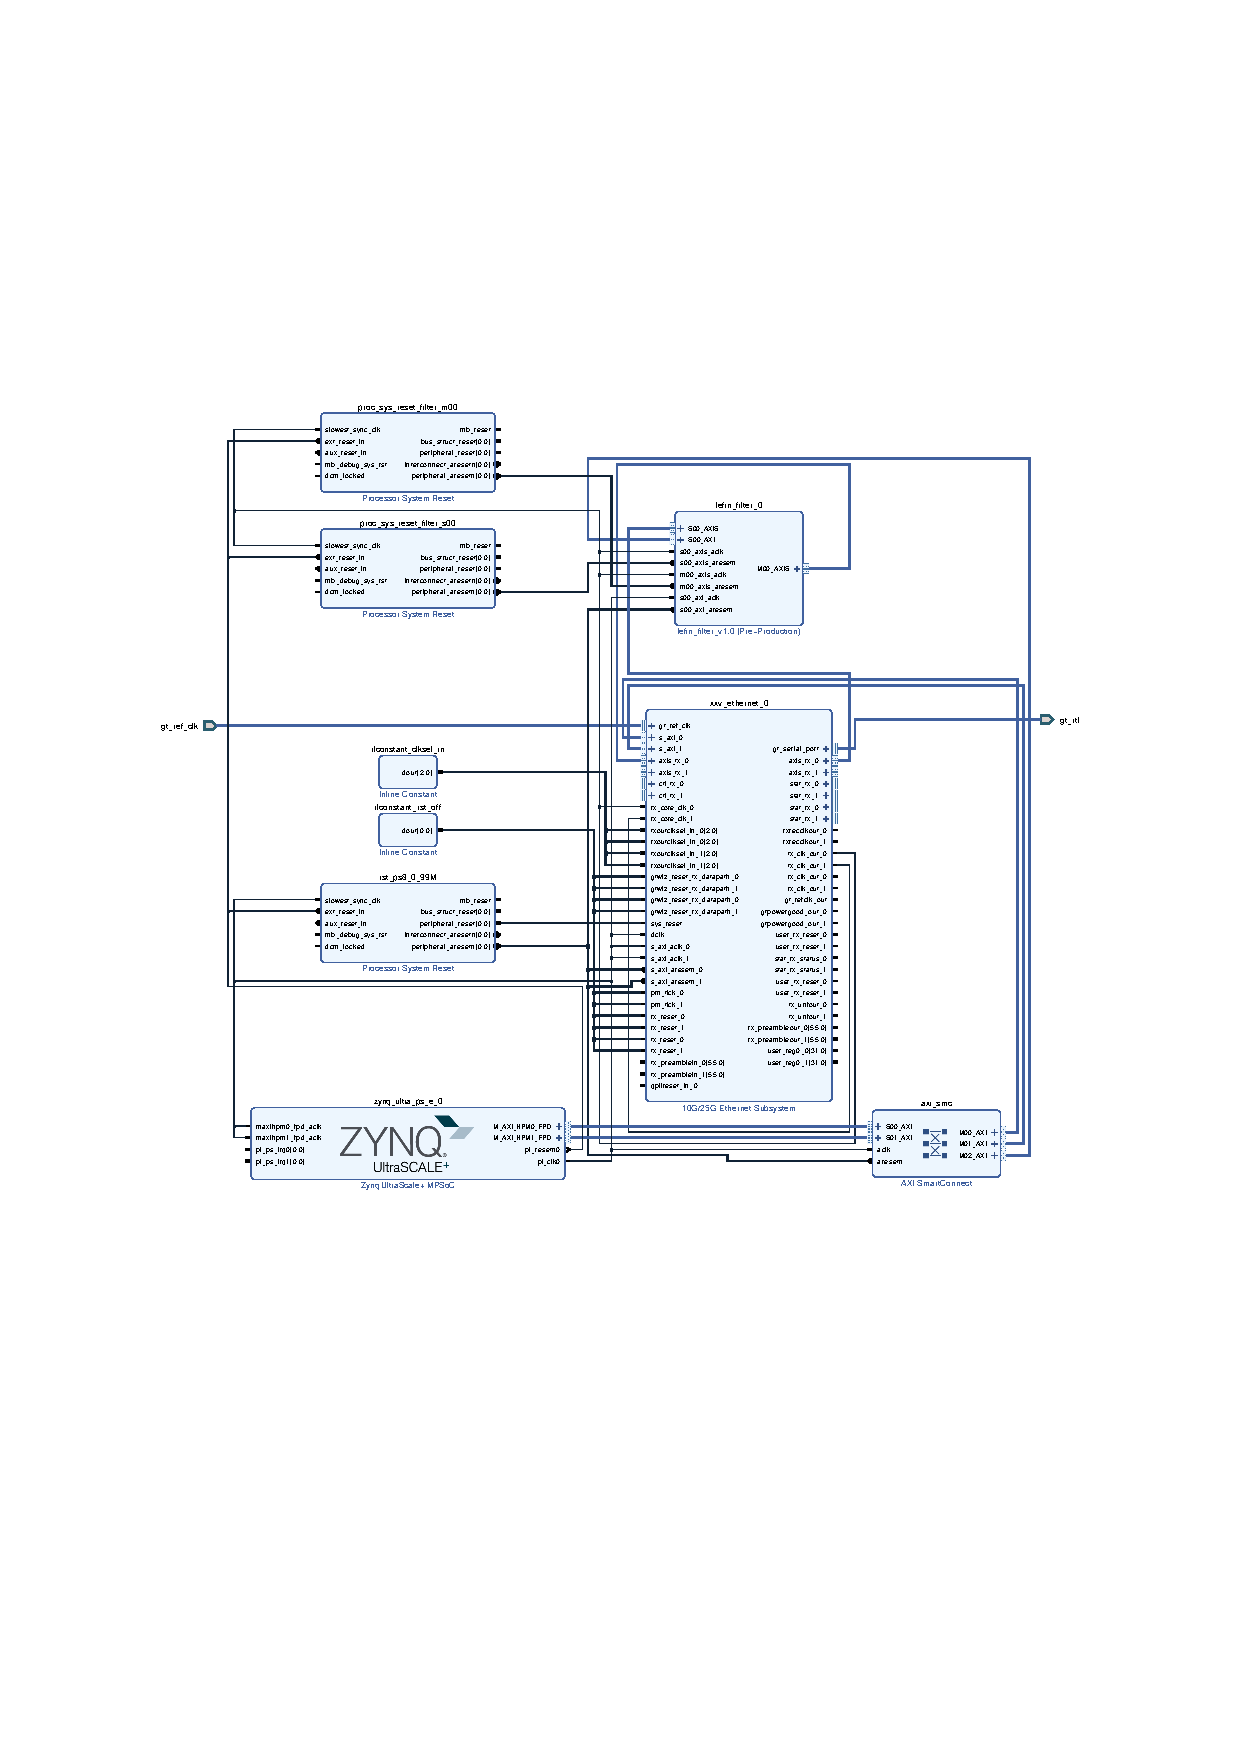
\includegraphics[width=1\textwidth, trim={0 9cm 0 6cm},clip]{images/block_diagram.pdf}
    \caption{LEFIN-Filter design block diagram}
    \label{fig:integration-block-diagram}
\end{figure*}

\end{document}

What is ethernet, background on networking and management, background on encryption (per process encrypted but in a way that can give away what type of process it is i.e. gmail, bittorrent, malware), what should be done with a bad packet, does that affect other flows? research paper, model architecure, challenges with typical ml pipeline for this classification baseline results?, why we think fpga would be good for this, QSFP

\subsection{Goals}
total accuracy, accuracy compared to model, latency, speed, design requirements, space requirements, clock to use, ports to use, not rely on too much ip
